\chapter{Conclusion} \label{chap:4}
    
    As of today, VeGETA is still in version v0.3 (alpha) and, therefore, not in the final release state. Using VeGETA in the proposed pipeline, without subsetting the data to reduce the necessary computation power, may result in ram overflow errors at the moment, especially when using the prediction of secondary structures function of VeGETA. However, there are improvements made every day and the overall clustering quality of VeGETA seems to be promising, as described in the project and visualized in \autoref{fig:3.7} for \gls{IBV}. Therefore, it seems to be useful to repeat the rating with full datasets of the \gls{IBV} segments using VeGETAs clustering alone or as described in the pipeline following by the secondary structure prediction at some point in the future and compare the results again. %Repetition with the segments of \gls{ICV} is not necessary, as there are less then 500 sequences in all the segment FASTA files and therefore all available data was already used. Having said that, the difference in the sequences of the \gls{ICV} segments are negligible and all three tools are creating three clusters at maximum, making the rating of these clusters not that meaningful for the aimed comparison of VeGETA and usearch or CD-HIT.
    
    The rating process used in this project was created to enable comparisons based on sequence difference with translation to \glspl{AA} in mind. But as already mentioned, for the final validation of the results, it may be necessary to repeat the rating with other concepts, like using the evolutionary distance, instead of the nucleotide to nucleotide comparisons and compare these rating approaches for even results. Furthermore, future use of better weighting approaches related to the single sequence clusters of the rating pipeline may be useful. 
    %Repeating the clustering of usearch and CD-HIT with different identity thresholds can be useful to, to compare VeGETAs clustering with different sequence identity settings of usearch and CD-HIT, because eventually the rating is done on the representatives and clusters sequence.

    %Furthermore more extensive substitution matrices can be used by modifying the pipeline to accept lookup tables for more sensitive differences. 
    For better validation of predicted secondary structures, it may be useful to repeat the pipeline with \gls{IAV} segments and a later version of VeGETA. Structures for segments of \gls{IAV} generated by \textit{in vivo} probing \autocite{probing} and generated by \textit{in silico} prediction were published already \autocite{A_structure1, A_structure2, A_structure3} and can be used for comparison.
    
    The use of fully assembled pseudogenomes of the Influenza species can be another approach to search for secondary structures between the segments instead of inside them. At the moment, VeGETA is only able to calculate structures on the positive strand but this may change in near future. On top of that, the assembly of all combinations of \gls{IAV} segments by iteration is nearly a computationally impossible task. To assemble only the proven and existing combinations in a reasonable amount of time can still be accomplished, by using a pipeline which utilizes the advantages of databases. Using joins, the segments in the database can be assembled to build the existing genome combinations and using VeGETA on this resulting FASTA file. Even with version v0.3 (alpha) and the positive strands only, many possible structures were found in the existing pseudogenomes of \gls{ICV} assembled that way (\autoref{fig:4.2}).
    
    \begin{figure}[!htb]
        \centering
        \fbox{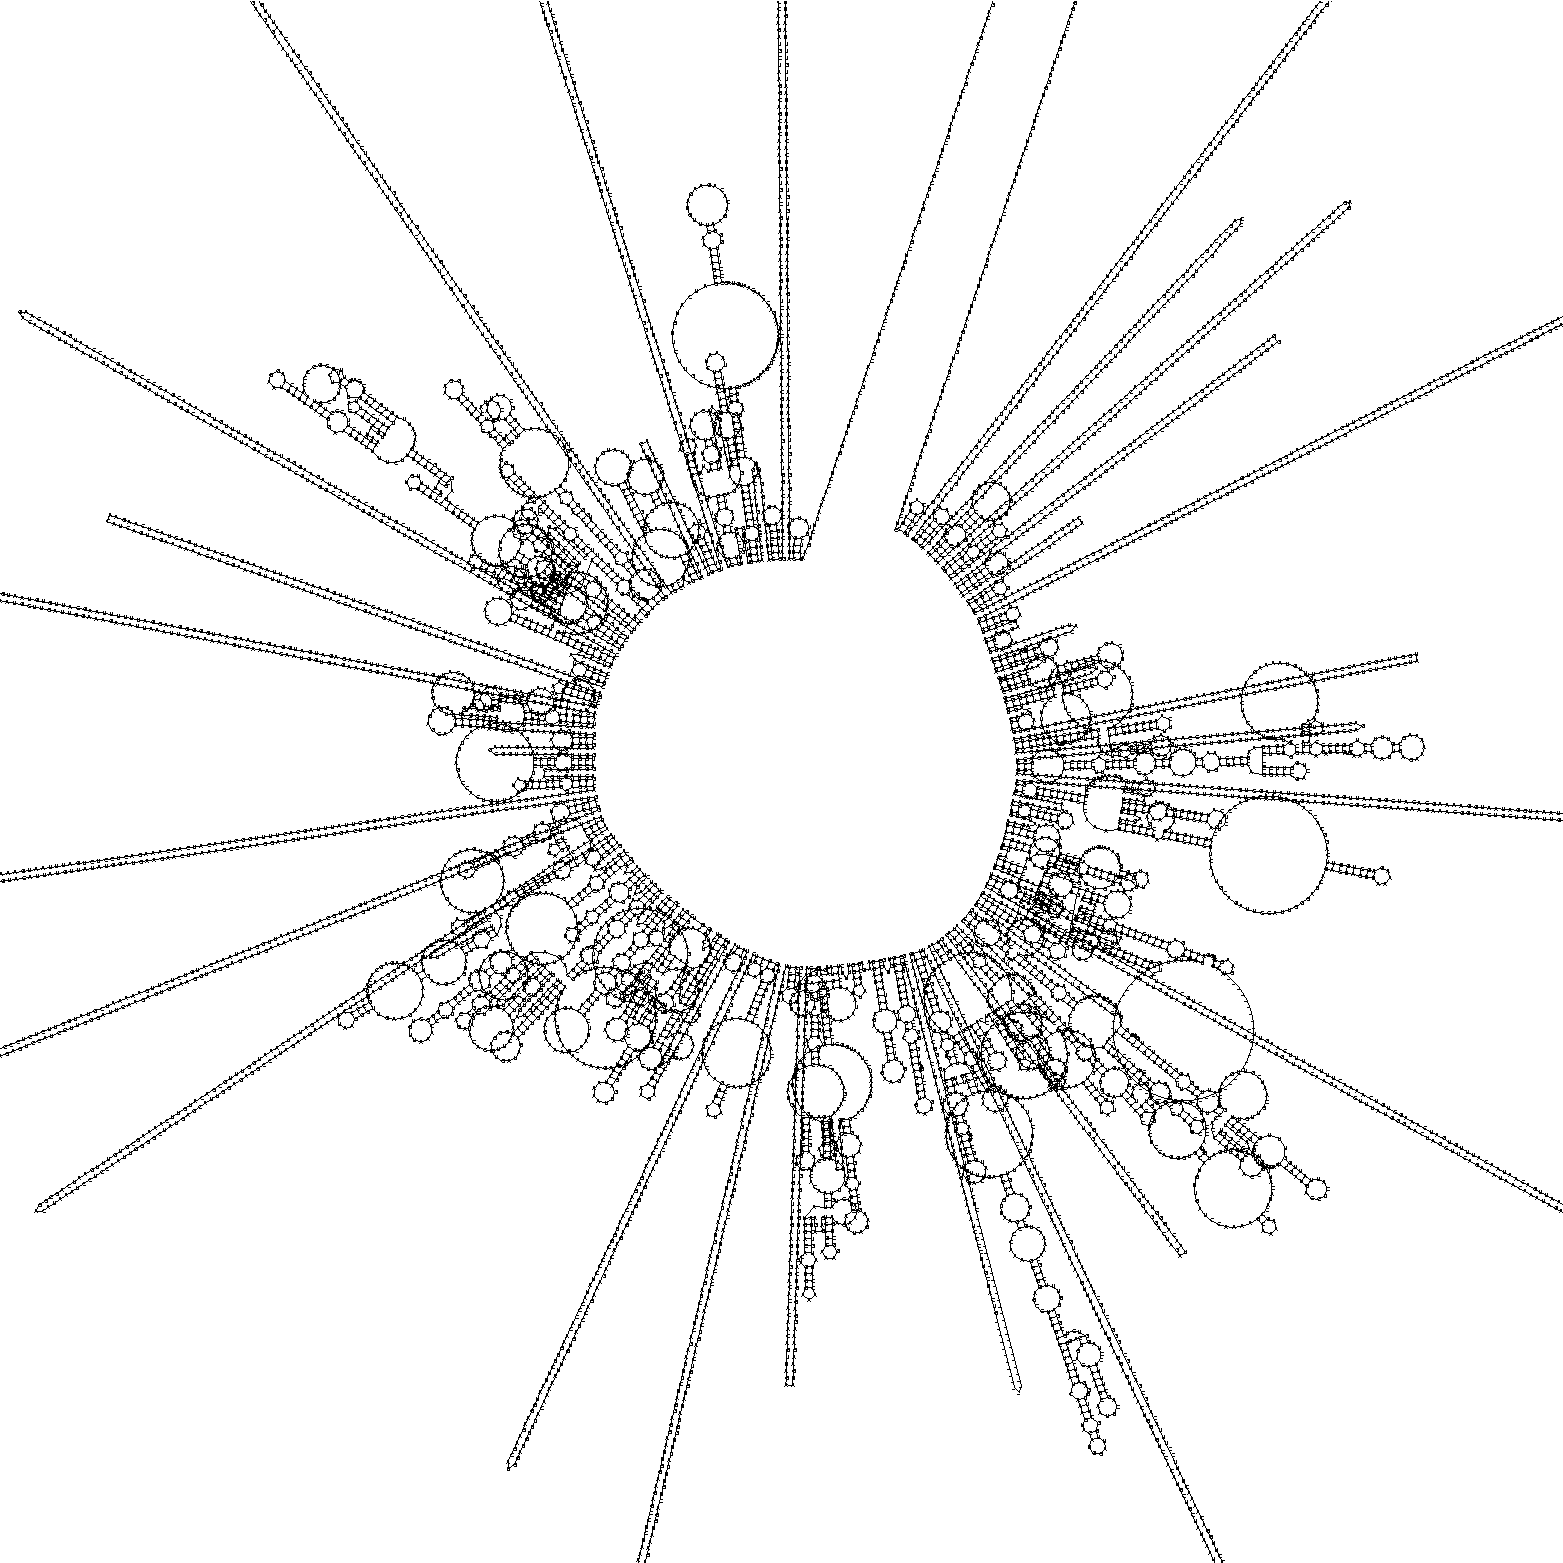
\includegraphics[width=\dimexpr\textwidth-2\fboxsep-2\fboxrule]{Figures/C_query.pdf}}
        \caption[Structures of the pseudogenomes of \gls{ICV}]{\textbf{Structures of the pseudogenomes of \gls{ICV}.} Secondary structures found by running VeGETA on the existing sequence combination (pseudogenomes) of \gls{ICV}. Most secondary structures were still predicted inside the segments instead of between, but this correspond with the only possible use of positive sequences by VeGETA at the moment.}
        \label{fig:4.2}
    \end{figure}
    
% \textbf{intro}
% \begin{itemize}[noitemsep]
%     \item Influenze ABC 
%     \item Cluster algorithmenn nennen inf a zu groß für clustern
%     \item bäume etc 
%     \item link github repo vegeta zitat
%     \item wann cluster gut? rating
%     \item cdhit usearch populär kmer vegeta
%     \item vegeta???
%     \item umap hdbscan k-mer basiert 1-2 sätze
%     \item zitate
%     \item clusterin paper reinschrieben!!!
% \end{itemize}

% \textbf{material \& methods}
% \begin{itemize}[noitemsep]
%     \item datum download ird
%     \item beim ersten nennne tool zitat parameter und versiopn holy trin
% \end{itemize}

% \textbf{results \& discussion}
% \begin{itemize}[noitemsep]
%     \item pipeline
%     \item rating implementiert laufzeit wie lange gebraucht
%     \item manhatten win size step gucken vergleich
%     \item rating auf sequenzbasis
%     \item clustering sequenzidentität cd hit usearch besser wenig variation in der sequenz aber daüfr evolutionär komisch, clustern auf evolutionärer basis besser?
%     \item vegeta wensentlich feineres cluster
%     \item influenza schwierig zu clustern reassortment etc nicht grade aussagekräftig
%     \item usearch und cdhit selbe parameter, VeGETA anders
%     \item 3er 3er codon step size
%     \item barplot
%     \item cluster distant metric substitution etc paper
%     \item pitfalls beim clustern ? wie gut ist ein cluster paper ? finden?
%     \item gewichten?????
%     \item implementieren?
%     \item nur eine coole struktur weil cgut geclustert
%     \item ss und amino cool ? durch clustern erhalten 
%     \item erweitern pipeline mafft auf centroids
% \end{itemize}

% \textbf{conclusion}
% \begin{itemize}[noitemsep]
%     \item Rating rating rating
%     \item secondary structure
%     \item Ausblick komplette gemome nutzen
%     \item Part II ?
%     \item metriken raxml matrizen referenz
%     \item database
%     \item was durchs rating gelernt reicht codon triplet nur distanz scheiße blabla
%     \item nucleotide awareness wichtig?
%     \item inf a to big
%     \item robustness
%     \item distanz gut? normailisieren kombinieren mit evolutionär
%     \item blabla 
%     \item masterarbeit
%     \item struktut auf sequenz 
% \end{itemize}


    